\documentclass{article}
  %----------------------------------------------------------------------------------------
%	Author:	WangYifu
%	Create Date:	2017-02-14
%	Last Modify:	2018-09-01
%----------------------------------------------------------------------------------------
\usepackage[T1]{fontenc}
\usepackage{fourier}
\usepackage[english]{babel}
\usepackage{amsmath,amsfonts,amsthm}
\usepackage{geometry}
\usepackage{fancyhdr}
\usepackage{listings}
\usepackage{color}
\usepackage[yyyymmdd]{datetime}
\usepackage{graphicx}
\usepackage{float}
\usepackage{titling}
\usepackage{titlesec}
%-------------------------------%
%          Page Style           %
%-------------------------------%
\pagestyle{fancyplain}
\fancyhead{}
\fancyfoot[L]{}
\fancyfoot[C]{}
\fancyfoot[R]{\thepage}
\renewcommand{\headrulewidth}{0pt}
\renewcommand{\footrulewidth}{0pt}
\setlength{\headheight}{13.6pt}
\textwidth=6.5in
\textheight=9.0in
\headsep = 0.1in
\renewcommand{\baselinestretch}{1.2}
\geometry{a4paper,left=2cm,right=2cm,top=2cm,bottom=2cm}

%-------------------------------%
%           Font Size           %
%-------------------------------%
\newcommand{\erhao}{\fontsize{22.1pt}{\baselineskip}\selectfont}
\newcommand{\sanhao}{\fontsize{16.1pt}{\baselineskip}\selectfont}
\newcommand{\sihao}{\fontsize{14.1pt}{\baselineskip}\selectfont}
\newcommand{\xiaosi}{\fontsize{12.1pt}{\baselineskip}\selectfont}
\newcommand{\wuhao}{\fontsize{10.5pt}{\baselineskip}\selectfont}
\newcommand{\setFontSize}[1]{\fontsize{#1}{\baselineskip}\selectfont}
\titleformat{\section}{\sanhao\bfseries}{$\bullet$}{5pt}{}

%-------------------------------%
%             Title             %
%-------------------------------%
\newcommand{\horrule}[1]{\rule{\linewidth}{#1}}
\renewcommand{\dateseparator}{ - }
\def\Assignment{Assignment Title}
\title{
\vspace{-2cm}
\normalfont \normalsize
\textsc{Washington University in St. Louis} \\ [0pt]
\horrule{1pt} \\[0.4cm]
\huge {\bf\Assignment}
}
\author{467261 - Yifu Wang}
\date{\normalsize\today\\\horrule{1pt} \\[0.5cm]}

%-------------------------------%
%           TableList           %
%-------------------------------%
\newcommand{\deflabel}[1]{#1\hfill}
\newenvironment{tlist}[1]{
	\begin{list}{}{
			\settowidth{\labelwidth}{\bf#1}
			\setlength{\leftmargin}{\labelwidth}
			\addtolength{\leftmargin}{\labelsep}
			\renewcommand{\makelabel}{\bf\deflabel}}}{
	\end{list}
}

%-------------------------------%
%             Code              %
%-------------------------------%
\definecolor{gray}{RGB}{191,191,191}
\definecolor{dkgreen}{RGB}{96,139,78}
\definecolor{mauve}{RGB}{206,145,120}

\lstset{ %
	language=C++,                % the language of the code
	% basicstyle=\textheight,           % the size of the fonts that are used for the code
	numbers=left,                   % where to put the line-numbers
	numberstyle=\color{black},  % the style that is used for the line-numbers
	stepnumber=0,                   % the step between two line-numbers. If it's 1, each line 
	% will be numbered
	numbersep=5pt,                  % how far the line-numbers are from the code
	backgroundcolor=\color{gray},      % choose the background color. You must add \usepackage{color}
	showspaces=false,               % show spaces adding particular underscores
	showstringspaces=false,         % underline spaces within strings
	showtabs=false,                 % show tabs within strings adding particular underscores
	frame=false,                   % adds a frame around the code
	rulecolor=\color{gray},        % if not set, the frame-color may be changed on line-breaks within not-black text (e.g. commens (green here))
	tabsize=2,                      % sets default tabsize to 2 spaces
	captionpos=b,                   % sets the caption-position to bottom
	breaklines=true,                % sets automatic line breaking
	breakatwhitespace=false,        % sets if automatic breaks should only happen at whitespace
	keywordstyle=\color{blue},          % keyword style
	commentstyle=\color{dkgreen},       % comment style
	stringstyle=\color{mauve},         % string literal style
}

  \def\Assignment{CES571S - L3 - MD5 Collision}
\begin{document}
\maketitle
\section{Generating Two Different Files with the Same MD5 Hash}
\subsection{Question 1}
Create a \code{prefix.txt} file with 63 byte.
\begin{figure}[H]\centering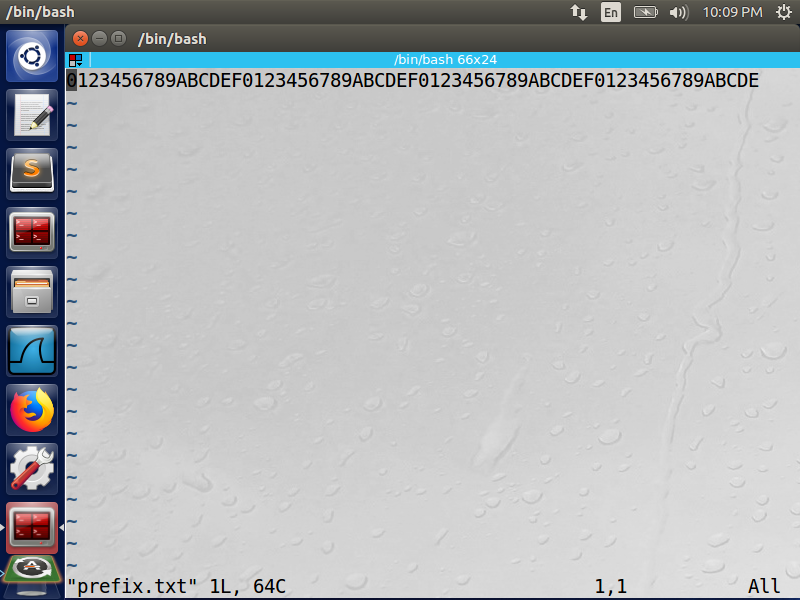
\includegraphics[width=\textwidth]{ss/01.png}\end{figure}
Using \code{md5collgen} tool, successfully generated 2 output binary files.
\begin{figure}[H]\centering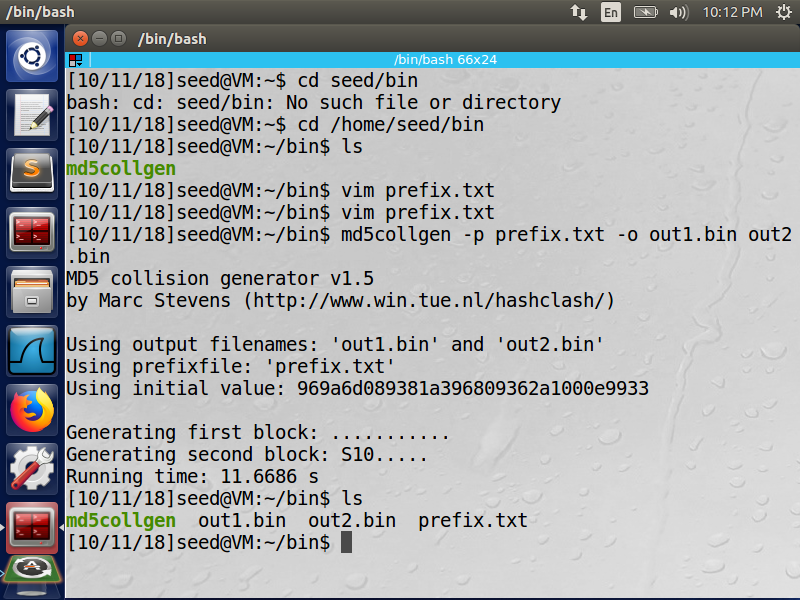
\includegraphics[width=\textwidth]{ss/02.png}\end{figure}
We can see that although \code{out1.bin} differs from \code{out2.bin}. Their MD5 are identital.
\begin{figure}[H]\centering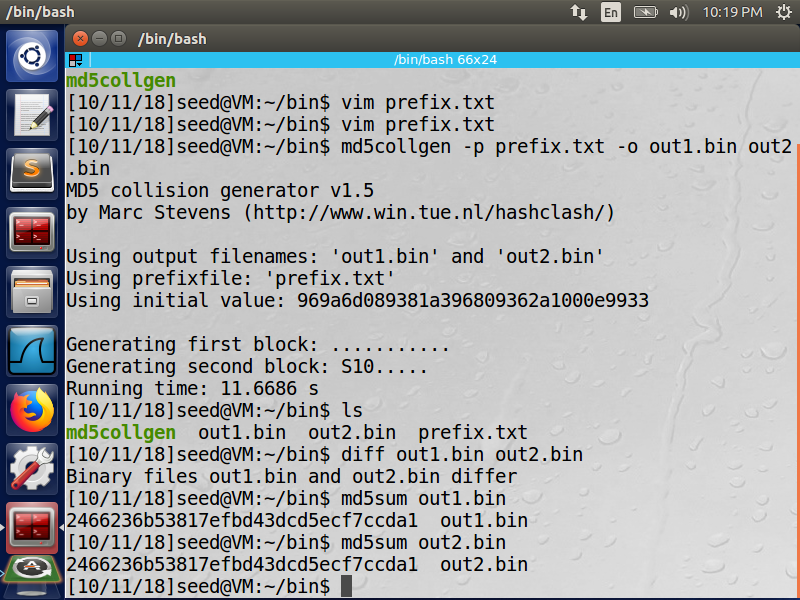
\includegraphics[width=\textwidth]{ss/03.png}\end{figure}
\subsection{Question 2}
Using a prefix file with exactly 64 byte.
\begin{figure}[H]\centering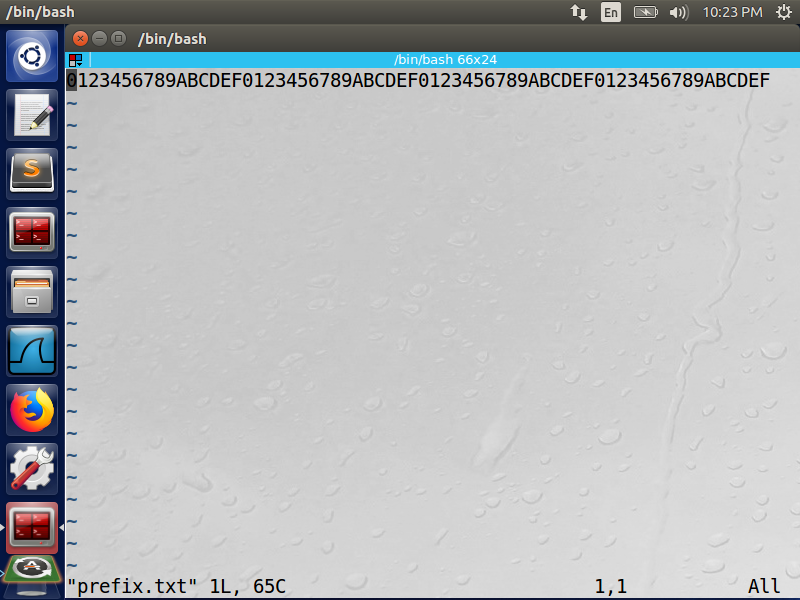
\includegraphics[width=\textwidth]{ss/04.png}\end{figure}
The result will be
\begin{figure}[H]\centering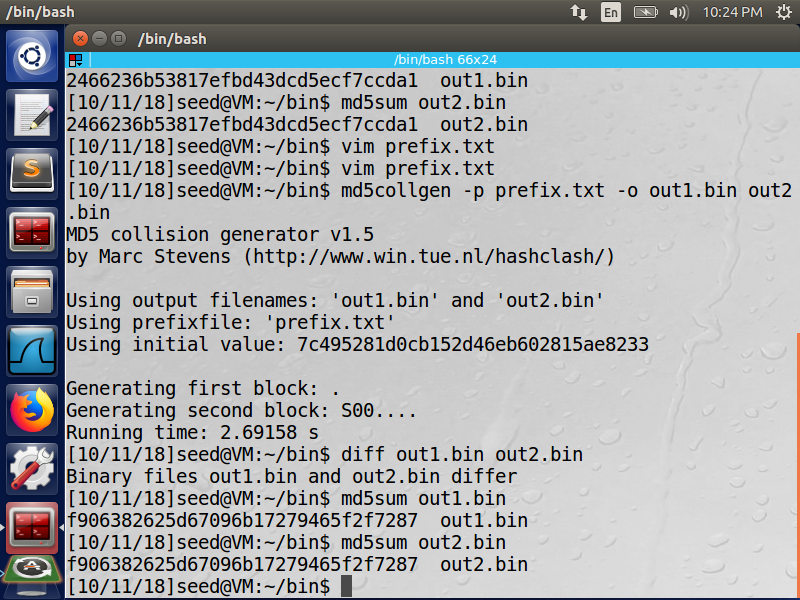
\includegraphics[width=\textwidth]{ss/05.png}\end{figure}
The \code{out1.bin} differs \code{out2.bin} but their MD5 are same just like the result in Question 1. But the generating process are a little different. In first question it took most of its time to generate first block and took 11s in total. But in second question it generated the first block immediately and tooks 2.6s in total.
\subsection{Question 3}
Most of them are same only few bytes are different. And after repeat this process I find all the different byte in those outputs seem to be exactly the same. That is in the last 128 byte(the appended section), the 20th, the 60th, the 84th, the 110th and the 124th byte are different(5 bytes in total).
\begin{figure}[H]\centering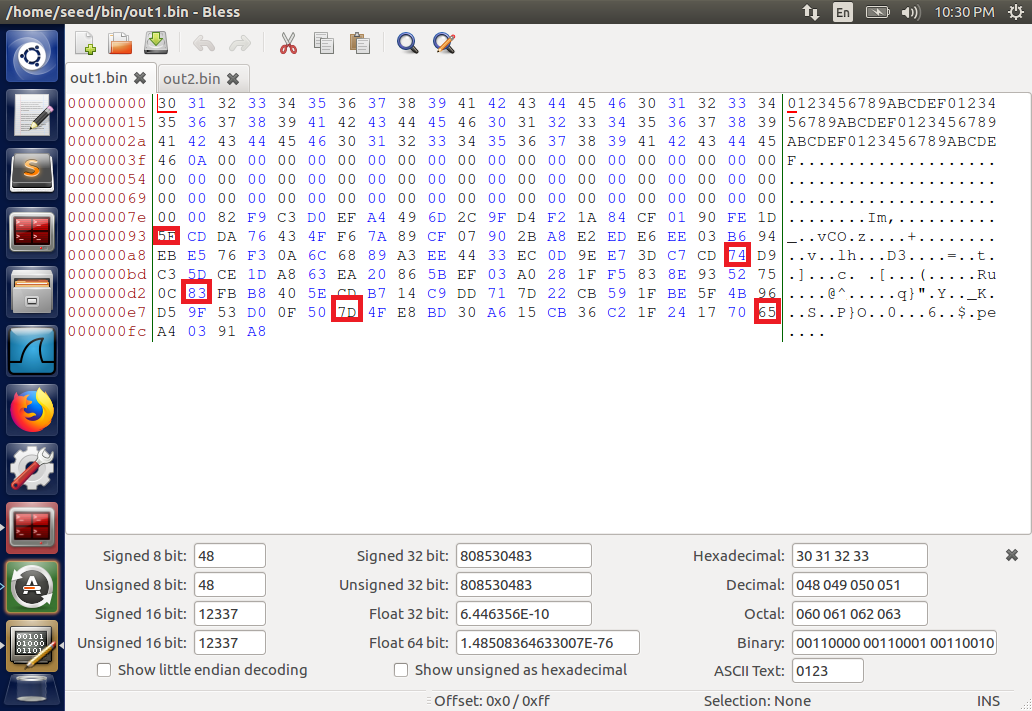
\includegraphics[width=\textwidth]{ss/06.png}\end{figure}
\begin{figure}[H]\centering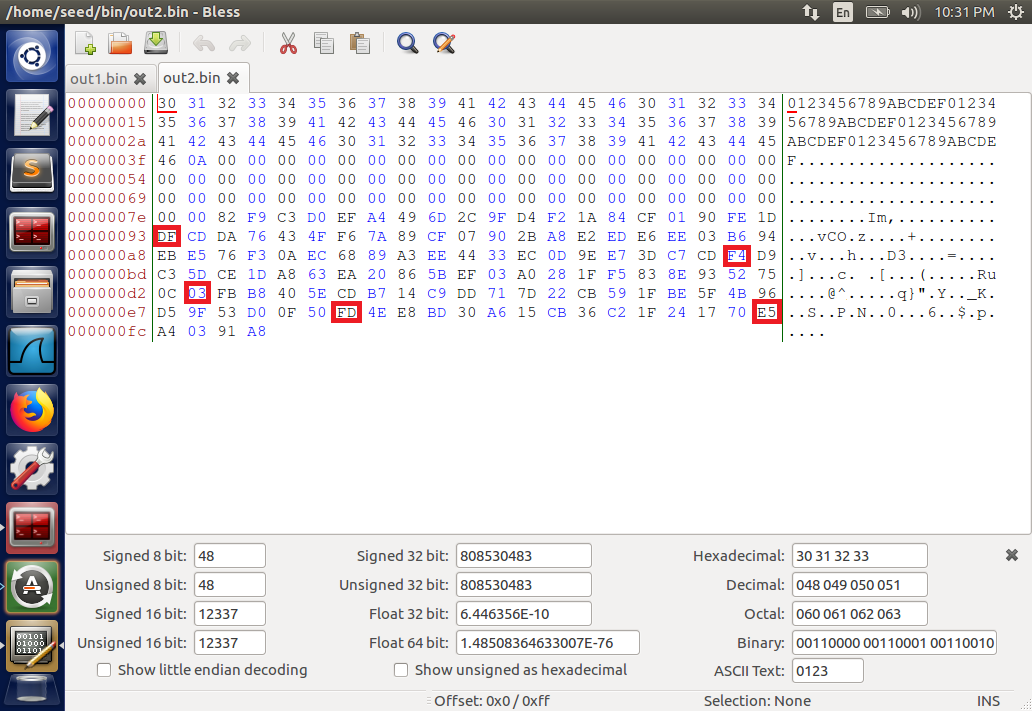
\includegraphics[width=\textwidth]{ss/07.png}\end{figure}
\section{Understanding MD5's Property}
So I will use the 3 file in the first task to varify this property. Since \code{MD5(out1.bin)=MD5(out2.bin)}. I will concatenate them with a random file, like \code{prefix.txt}.
\begin{figure}[H]\centering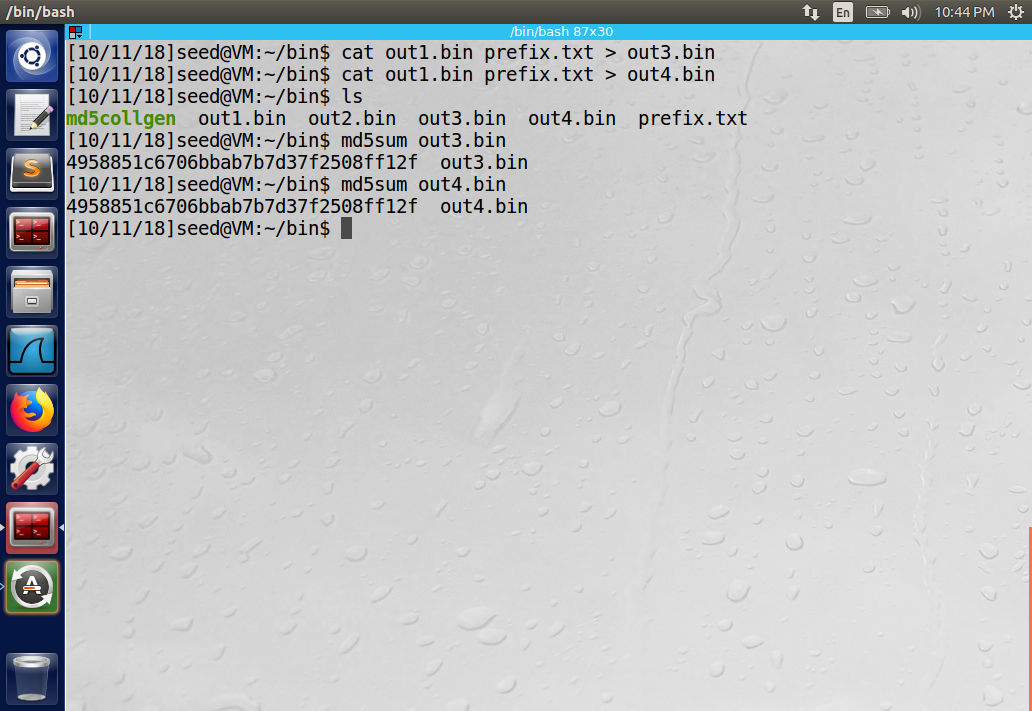
\includegraphics[width=\textwidth]{ss/08.png}\end{figure}
According to the \code{md5sum} results. This property holds for MD5.
\section{Generating Two Executable Files with the Same MD5 Hash}
Firstly create the following \code{src.c} C source code.
\begin{figure}[H]\centering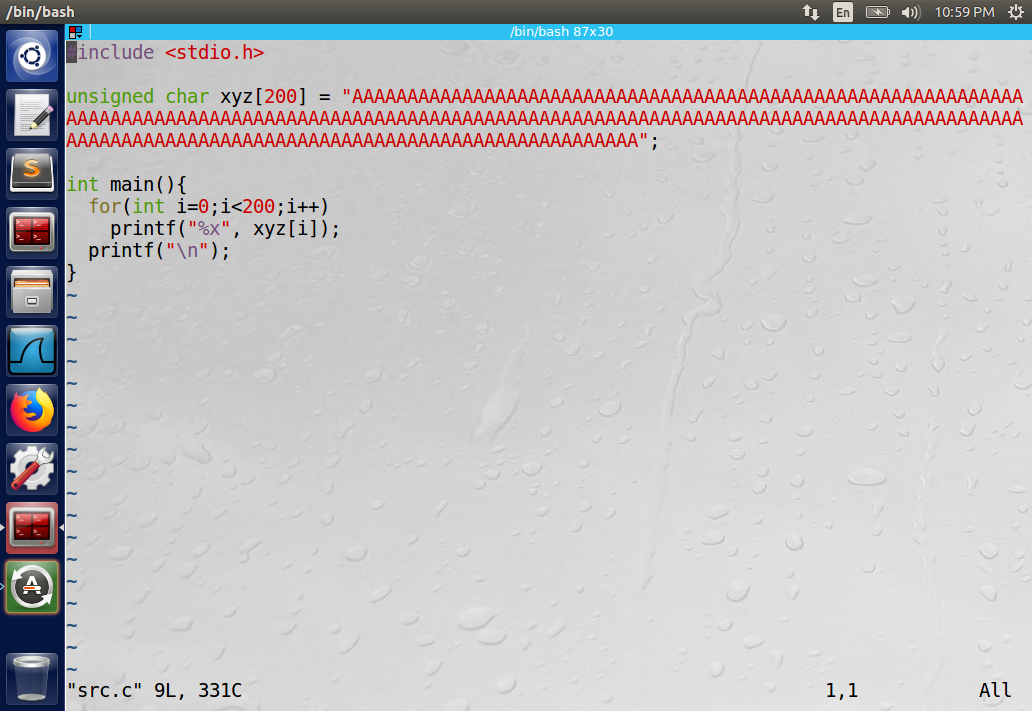
\includegraphics[width=\textwidth]{ss/09.png}\end{figure}
Then compile it using \code{gcc}, and run it to see the normal result.
\begin{figure}[H]\centering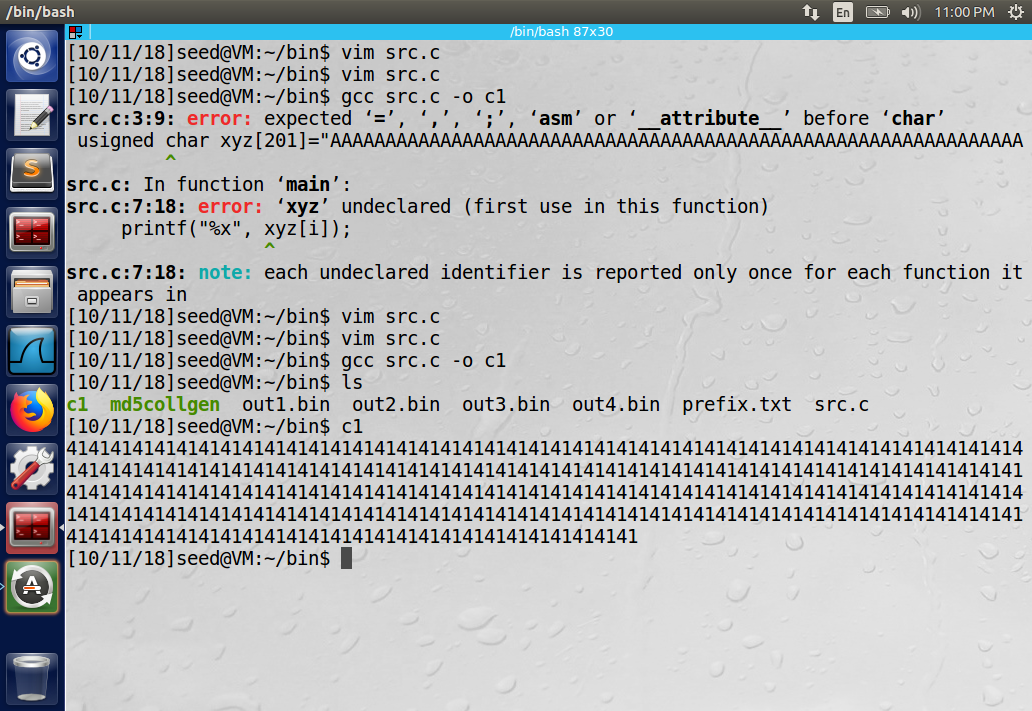
\includegraphics[width=\textwidth]{ss/10.png}\end{figure}
Open \code{c1} using \code{bless} and find a prefix fit our need (nultiple of 64 and locate inside the string). You can see 4160 is mutiple of 64 and inside the string.
\begin{figure}[H]\centering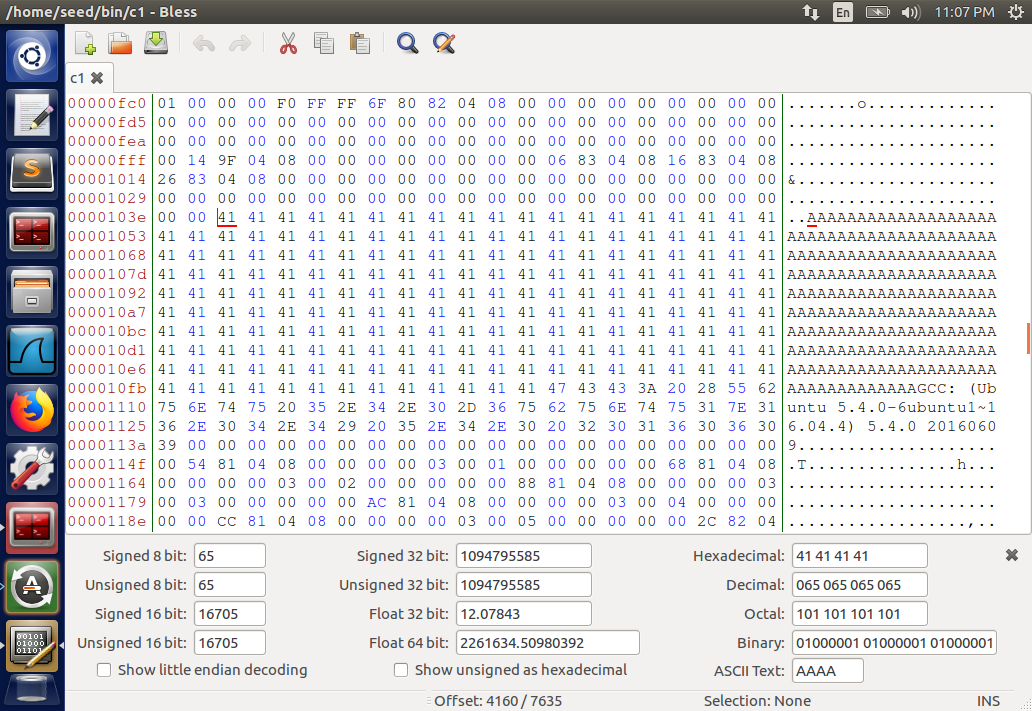
\includegraphics[width=\textwidth]{ss/11.png}\end{figure}
Thus we cut the prefix and suffix from 4160 and +4289. Then compute P and Q with \code{md5collgen}, and recat them together. Here, be awared that \code{md5collgen} products all ready include the prefix you provided. And in order to execute the modified binary file, you need to use command \code{chmod +x}.
\begin{figure}[H]\centering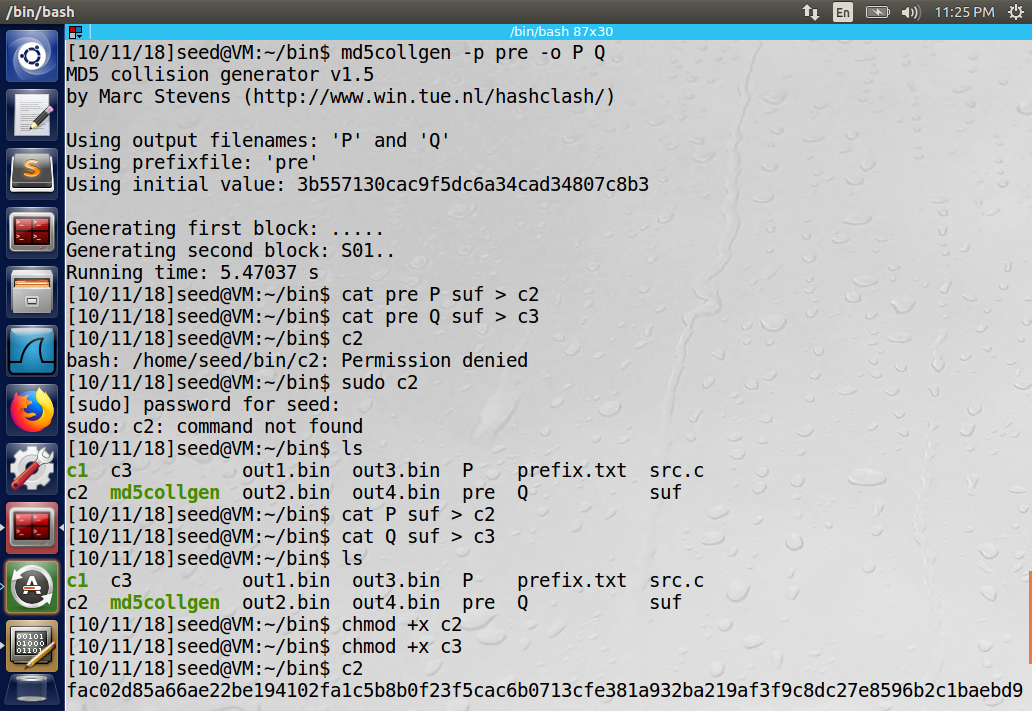
\includegraphics[width=\textwidth]{ss/12.png}\end{figure}
Then run them to see different result, and verify their MD5s are identical.
\begin{figure}[H]\centering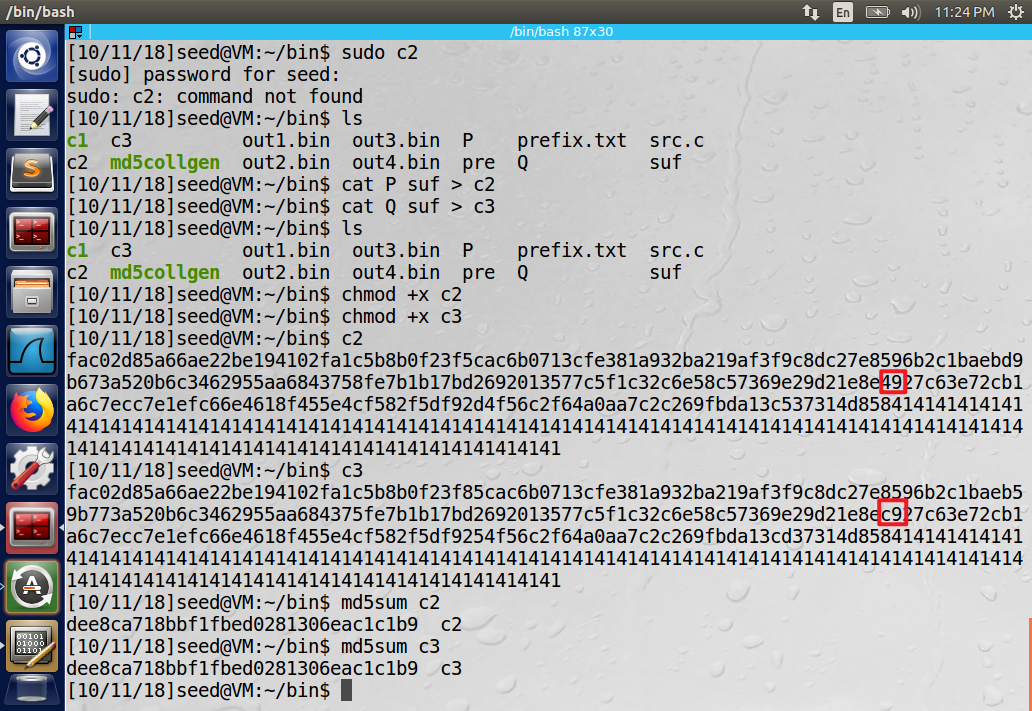
\includegraphics[width=\textwidth]{ss/13.png}\end{figure}
There are multiple bytes different but I only marked one of them.
\section{Making the Two Programs Behave Differently}
Based on my observation in Task 1 Question 3, I think I can just compare the 20th byte of the differtent section to check if our program should pretend to be good or act bad. To achieve this we need to know the exactly position where the judgement statement is executed. But I assume change the code behind the declaration of our array will not change the code before. So I wrote the code as
\begin{figure}[H]\centering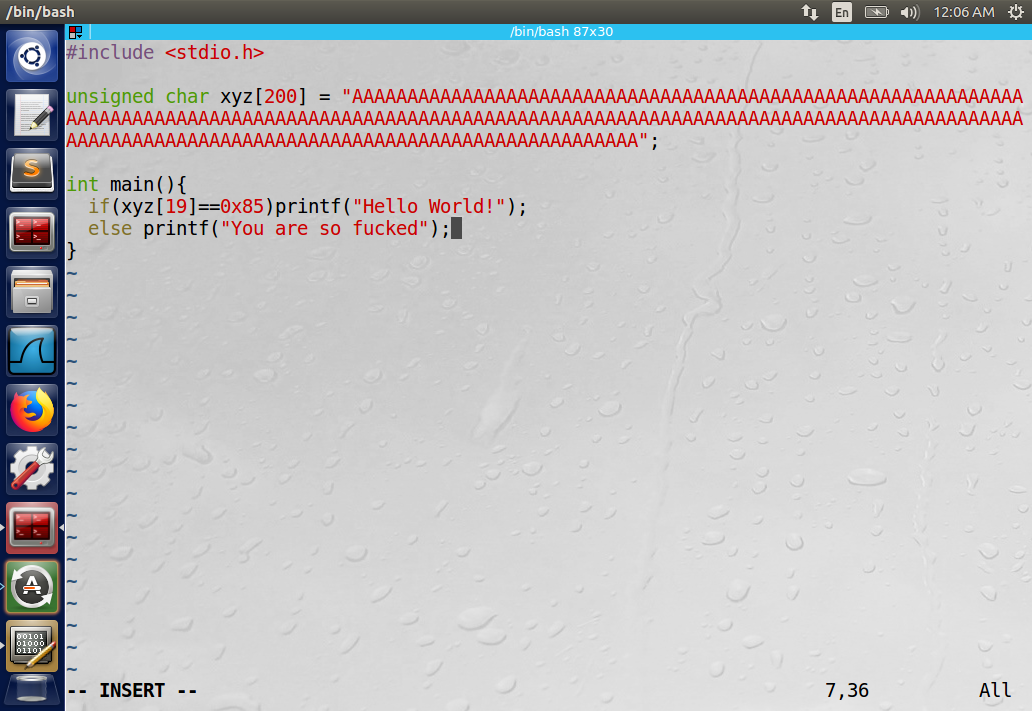
\includegraphics[width=\textwidth]{ss/14.png}\end{figure}
Then repeat the process described in task 3 here is the result.
\begin{figure}[H]\centering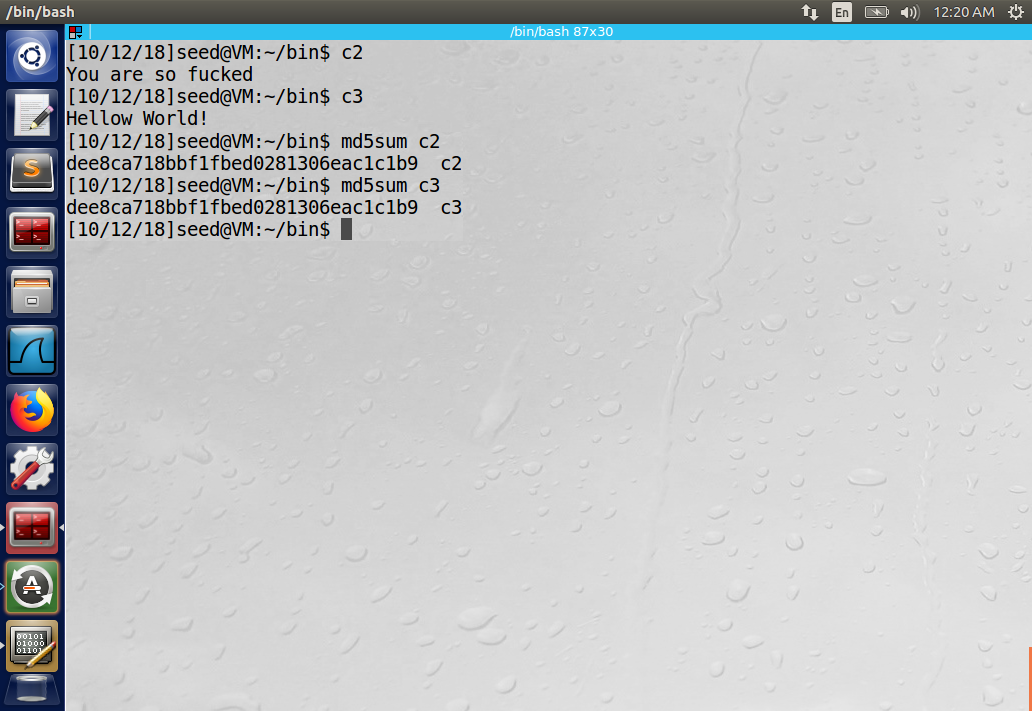
\includegraphics[width=\textwidth]{ss/15.png}\end{figure}
You can see those two program has totally different behavior. Although they only print different 'meaningful' text in this case, but it can actually do any thing they want.
\end{document}